 \documentclass[12pt,a4paper]{article}
\usepackage{hyperref} % Use the Charter font for the document text
%\usepackage[UTF8]{ctex}
\usepackage{fullpage}
\usepackage{amsfonts,amssymb,amsmath}
\usepackage{mathtools}
\usepackage{tikz-cd}
\usepackage{tikz}

\usepackage{alltt}
\usepackage{amsfonts}
\usepackage{amsmath}
\usepackage{amssymb}
\usepackage{amsthm}
\usepackage{booktabs}
\usepackage{caption}
\usepackage{enumitem}
\usepackage{fancyhdr}
\usepackage{graphicx}
\usepackage{mathdots}
\usepackage{mathtools}
\usepackage{microtype}
\usepackage{multirow}
\usepackage{pdflscape}
\usepackage{pgfplots}
\usepackage{siunitx}
\usepackage{slashed}
\usepackage{tabularx}
\usepackage{tikz}
\usepackage{tkz-euclide}
\usepackage[normalem]{ulem}
\usepackage[all]{xy}
\usepackage{imakeidx}

\newcommand{\bA}{\ensuremath{\mathbb{A}}}
\newcommand{\bB}{\ensuremath{\mathbb{B}}}
\newcommand{\bC}{\ensuremath{\mathbb{C}}}
\newcommand{\bD}{\ensuremath{\mathbb{D}}}
\newcommand{\bE}{\ensuremath{\mathbb{E}}}
\newcommand{\bF}{\ensuremath{\mathbb{F}}}
\newcommand{\bG}{\ensuremath{\mathbb{G}}}
\newcommand{\bH}{\ensuremath{\mathbb{H}}}
\newcommand{\bI}{\ensuremath{\mathbb{I}}}
\newcommand{\bJ}{\ensuremath{\mathbb{J}}}
\newcommand{\bK}{\ensuremath{\mathbb{K}}}
\newcommand{\bL}{\ensuremath{\mathbb{L}}}
\newcommand{\bM}{\ensuremath{\mathbb{M}}}
\newcommand{\bN}{\ensuremath{\mathbb{N}}}
\newcommand{\bO}{\ensuremath{\mathbb{O}}}
\newcommand{\bP}{\ensuremath{\mathbb{P}}}
\newcommand{\bQ}{\ensuremath{\mathbb{Q}}}
\newcommand{\bR}{\ensuremath{\mathbb{R}}}
\newcommand{\bS}{\ensuremath{\mathbb{S}}}
\newcommand{\bT}{\ensuremath{\mathbb{T}}}
\newcommand{\bU}{\ensuremath{\mathbb{U}}}
\newcommand{\bV}{\ensuremath{\mathbb{V}}}
\newcommand{\bW}{\ensuremath{\mathbb{W}}}
\newcommand{\bX}{\ensuremath{\mathbb{X}}}
\newcommand{\bY}{\ensuremath{\mathbb{Y}}}
\newcommand{\bZ}{\ensuremath{\mathbb{Z}}}


%
%\parskip=1em
%\parindent=0.3in
%\setlength\oddsidemargin{0.5in} \setlength\evensidemargin{0.5in}
%\setlength\textwidth{5.5in}
%
%\hfuzz6pt % Don't bother to report over-full boxes if over-edge is < 6pt
%
%\newlength{\defbaselineskip}
%\setlength{\defbaselineskip}{\baselineskip}
%\newcommand{\setlinespacing}[1]%
%           {\setlength{\baselineskip}{#1 \defbaselineskip}}
%\newcommand{\doublespacing}{\setlength{\baselineskip}%
%                           {2.0 \defbaselineskip}}
%\newcommand{\singlespacing}{\setlength{\baselineskip}{\defbaselineskip}}
%
%\newcommand{\properpagestyle}{\pagestyle{myheadings}\markboth{}{}\markright{}}




\def\Ric{\mathop{\rm Ric}}
\def\cRic{\mathop{\stackrel{\circ}{\Ric}}}
\def\Scal{\mathop{\rm R}}
\def\scL{\mathop{\mathcal L}}
\def\Hess{\mathop{\rm Hess}}
\def\bt{\mathop{\bar\tau}}
\def\dist{\mathop{\rm dist}}
\def\Cut{\mathop{\rm Cut}}
\def\Riem{\mathop{\rm Rm}}
\def\scal{\mathop{\rm scal}}
\def\Sec{\mathop{\rm Sec}}
\def\Diam{\mathop{\rm Diam}}
\def\CS{\mathop{\rm C_S}}
\def\V{\mathop{\rm V}}
\def\Vol{\mathop{\rm Vol}}
\def\Area{\mathop{\rm Area}}
\def\VR{\mathop{\rm VR}}
\def\supp{\mathop{\rm supp}}
\def\div{\mathop{\rm div}}
\def\inj{\mathop{\rm inj}}
\def\diam{\mathop{\rm diam}}
\def\Id{\mathop{\rm Id}}
\def\RRR{\mathop{\mathcal{R}}}
\def\MMM{\mathop{\mathcal{M}}}
\def\HHH{\mathop{\mathcal{H}}}
\def\VVV{\mathop{\mathcal{V}}}
\def\FF{\mathop{\mathbb{F}}}
\def\RR{\mathop{\mathbb{R}}}
\def\QQ{\mathop{\mathbb{Q}}}
\def\CC{\mathop{\mathbb{C}}}
\def\ZZ{\mathop{\mathbb{Z}}}
\def\SS{\mathop{\mathbb{S}}}
\def\SSS{\mathop{\mathcal{S}}}
\def\PP{\mathop{\mathbb{P}}}
\def\End{\mathop{\rm End}}
\def\Aut{\mathop{\rm Aut}}
\def\Ad{\mathop{\rm Ad}}
\def\ad{\mathop{\rm ad}}
\def\hht{\mathop{\rm ht}}
\def\gl{\mathop{\mathfrak{gl}}}
\def\ssl{\mathop{\mathfrak{sl}}}
\def\TP{\mathop{\mathcal{TP}}}
\def\PPP{\mathop{\mathcal{P}}}
\def\gggg{\mathop{\mathfrak{g}}}
\def\ffff{\mathop{\mathfrak{f}}}
\def\OO{\mathop{\mathcal{O}}}
\def\oo{\mathop{\mathfrak{o}}}
\def\GG{\mathop{\mathcal{G}}}
\def\WWW{\mathop{\mathcal{W}}}
\def\Rad{\mathop{\rm Rad}}
\def\Der{\mathop{\rm Der}}
\def\Ker{\mathop{\rm Ker}}
\def\Im{\mathop{\rm Im}}

\def\be{\begin{eqnarray}}
\def\ee{\end{eqnarray}}
\def\beg{\begin{eqnarray*}}
\def\ees{\end{eqnarray*}}


%\newcommand{\qed}{\hfill$\Box$}
\theoremstyle{definition}
\newtheorem*{aim}{Aim}
\newtheorem*{axiom}{Axiom}
\newtheorem*{claim}{Claim}
\newtheorem*{cor}{Corollary}
\newtheorem*{conjecture}{Conjecture}
\newtheorem*{defi}{Definition}
\newtheorem*{eg}{Example}
\newtheorem*{ex}{Exercise}
\newtheorem*{fact}{Fact}
\newtheorem*{law}{Law}
\newtheorem*{lemma}{Lemma}
\newtheorem*{notation}{Notation}
\newtheorem*{prop}{Proposition}
\newtheorem*{question}{Question}
\newtheorem*{thm}{Theorem}





% Maths symbols
\newcommand{\abs}[1]{\left\lvert #1\right\rvert}
%\newcommand\ad{\mathrm{ad}}
\newcommand\AND{\mathsf{AND}}
\newcommand\Art{\mathrm{Art}}
\newcommand{\Bilin}{\mathrm{Bilin}}
\newcommand{\bket}[1]{\left\lvert #1\right\rangle}
\newcommand{\B}{\mathcal{B}}
\newcommand{\bolds}[1]{{\bfseries #1}}
\newcommand{\brak}[1]{\left\langle #1 \right\rvert}
\newcommand{\braket}[2]{\left\langle #1\middle\vert #2 \right\rangle}
\newcommand{\bra}{\langle}
\newcommand{\cat}[1]{\mathsf{#1}}
\newcommand{\C}{\mathbb{C}}
\newcommand{\cU}{\mathcal{U}}
%\newcommand{\Der}{\mathrm{Der}}
\newcommand{\D}{\mathrm{D}}
\newcommand{\dR}{\mathrm{dR}}
\newcommand{\E}{\mathbb{E}}
\newcommand{\F}{\mathbb{F}}
\newcommand{\Frob}{\mathrm{Frob}}
%\newcommand{\GG}{\mathbb{G}}
%\newcommand{\gl}{\mathfrak{gl}}
\newcommand{\GL}{\mathrm{GL}}
\newcommand{\G}{\mathcal{G}}
\newcommand{\Gr}{\mathrm{Gr}}
\newcommand{\haut}{\mathrm{ht}}
\newcommand{\Hol}{\mathrm{Hol}}
\newcommand{\hol}{\mathfrak{hol}}
%\newcommand{\Id}{\mathrm{Id}}
\newcommand{\ket}{\rangle}
\newcommand{\lie}[1]{\mathfrak{#1}}
\newcommand{\Mat}{\mathrm{Mat}}
\newcommand{\N}{\mathbb{N}}
\newcommand{\norm}[1]{\left\lVert #1\right\rVert}
\newcommand{\normalorder}[1]{\mathop{:}\nolimits\!#1\!\mathop{:}\nolimits}
\newcommand{\NOT}{\mathsf{NOT}}
\newcommand{\op}{\mathrm{op}}
\newcommand{\Oc}{\mathcal{O}}
\newcommand{\Or}{\mathrm{O}}
\newcommand\OR{\mathsf{OR}}
\newcommand{\ort}{\mathfrak{o}}
\newcommand{\PGL}{\mathrm{PGL}}
\newcommand{\ph}{\,\cdot\,}
\newcommand{\pr}{\mathrm{pr}}
\newcommand{\Prob}{\mathbb{P}}
\newcommand{\PSL}{\mathrm{PSL}}
\newcommand{\Ps}{\mathcal{P}}
\newcommand{\PSU}{\mathrm{PSU}}
\newcommand{\pt}{\mathrm{pt}}
\newcommand{\qeq}{\mathrel{``{=}"}}
\newcommand{\Q}{\mathbb{Q}}
\newcommand{\R}{\mathbb{R}}
\newcommand{\Rs}{\mathcal{R}}
\newcommand{\SL}{\mathrm{SL}}
\newcommand{\so}{\mathfrak{so}}
\newcommand{\SO}{\mathrm{SO}}
\newcommand{\Spin}{\mathrm{Spin}}
\newcommand{\Sp}{\mathrm{Sp}}
\newcommand{\su}{\mathfrak{su}}
\newcommand{\SU}{\mathrm{SU}}
\newcommand{\term}[1]{\textbf{#1}\index{#1}}
\newcommand{\T}{\mathbb{T}}
\newcommand{\tv}[1]{|#1|}
\newcommand{\U}{\mathrm{U}}
\newcommand{\uu}{\mathfrak{u}}
\newcommand{\Vect}{\mathrm{Vect}}
\newcommand{\wsto}{\stackrel{\mathrm{w}^*}{\to}}
\newcommand{\wt}{\mathrm{wt}}
\newcommand{\wto}{\stackrel{\mathrm{w}}{\to}}
\newcommand{\Z}{\mathbb{Z}}
\renewcommand{\d}{\mathrm{d}}
\renewcommand{\H}{\mathbb{H}}
\renewcommand{\P}{\mathbb{P}}
\renewcommand{\sl}{\mathfrak{sl}}
\renewcommand{\vec}[1]{\boldsymbol{\mathbf{#1}}}
%\renewcommand{\F}{\mathcal{F}}

\let\Im\relax
\let\Re\relax

\DeclareMathOperator{\adj}{adj}
\DeclareMathOperator{\Ann}{Ann}
\DeclareMathOperator{\area}{area}
%\DeclareMathOperator{\Aut}{Aut}
\DeclareMathOperator{\Bernoulli}{Bernoulli}
\DeclareMathOperator{\betaD}{beta}
\DeclareMathOperator{\bias}{bias}
\DeclareMathOperator{\binomial}{binomial}
\DeclareMathOperator{\card}{card}
\DeclareMathOperator{\ccl}{ccl}
\DeclareMathOperator{\Char}{char}
\DeclareMathOperator{\ch}{ch}
\DeclareMathOperator{\cl}{cl}
\DeclareMathOperator{\cls}{\overline{\mathrm{span}}}
\DeclareMathOperator{\coker}{coker}
\DeclareMathOperator{\conv}{conv}
\DeclareMathOperator{\corr}{corr}
\DeclareMathOperator{\cosec}{cosec}
\DeclareMathOperator{\cosech}{cosech}
\DeclareMathOperator{\cov}{cov}
\DeclareMathOperator{\covol}{covol}
\DeclareMathOperator{\diag}{diag}
%\DeclareMathOperator{\diam}{diam}
\DeclareMathOperator{\Diff}{Diff}
\DeclareMathOperator{\disc}{disc}
\DeclareMathOperator{\dom}{dom}
%\DeclareMathOperator{\End}{End}
\DeclareMathOperator{\energy}{energy}
\DeclareMathOperator{\erfc}{erfc}
\DeclareMathOperator{\erf}{erf}
\DeclareMathOperator*{\esssup}{ess\,sup}
\DeclareMathOperator{\ev}{ev}
\DeclareMathOperator{\Ext}{Ext}
\DeclareMathOperator{\fst}{fst}
\DeclareMathOperator{\Fit}{Fit}
\DeclareMathOperator{\fix}{fix}
\DeclareMathOperator{\Frac}{Frac}
\DeclareMathOperator{\Gal}{Gal}
\DeclareMathOperator{\gammaD}{gamma}
\DeclareMathOperator{\gr}{gr}
\DeclareMathOperator{\hcf}{hcf}
\DeclareMathOperator{\Hom}{Hom}
\DeclareMathOperator{\id}{id}
\DeclareMathOperator{\Image}{image}
\DeclareMathOperator{\Im}{Im}
\DeclareMathOperator{\Ind}{Ind}
\DeclareMathOperator{\Int}{Int}
\DeclareMathOperator{\Isom}{Isom}
\DeclareMathOperator{\lcm}{lcm}
\DeclareMathOperator{\length}{length}
\DeclareMathOperator{\Lie}{Lie}
\DeclareMathOperator{\like}{like}
\DeclareMathOperator{\Lk}{Lk}
\DeclareMathOperator{\Maps}{Maps}
\DeclareMathOperator{\mse}{mse}
\DeclareMathOperator{\multinomial}{multinomial}
\DeclareMathOperator{\orb}{orb}
\DeclareMathOperator{\ord}{ord}
\DeclareMathOperator{\otp}{otp}
\DeclareMathOperator{\Poisson}{Poisson}
\DeclareMathOperator{\poly}{poly}
\DeclareMathOperator{\rank}{rank}
\DeclareMathOperator{\rel}{rel}
%\DeclareMathOperator{\Rad}{Rad}
\DeclareMathOperator{\Re}{Re}
\DeclareMathOperator*{\res}{res}
\DeclareMathOperator{\Res}{Res}
%\DeclareMathOperator{\Ric}{Ric}
\DeclareMathOperator{\rk}{rk}
\DeclareMathOperator{\Rees}{Rees}
\DeclareMathOperator{\Root}{Root}
\DeclareMathOperator{\sech}{sech}
\DeclareMathOperator{\sgn}{sgn}
\DeclareMathOperator{\snd}{snd}
\DeclareMathOperator{\Spec}{Spec}
\DeclareMathOperator{\spn}{span}
\DeclareMathOperator{\stab}{stab}
\DeclareMathOperator{\St}{St}
%\DeclareMathOperator{\supp}{supp}
\DeclareMathOperator{\Syl}{Syl}
\DeclareMathOperator{\Sym}{Sym}
\DeclareMathOperator{\tr}{tr}
\DeclareMathOperator{\Tr}{Tr}
\DeclareMathOperator{\var}{var}
\DeclareMathOperator{\vol}{vol}
\usetikzlibrary{knots}

\def\CY{Calabi--Yau}
\def\CP{\mathbb{C}\mathbf{P}}
\def\RP{\mathbb{R}\mathbf{P}}



\pgfarrowsdeclarecombine{twolatex'}{twolatex'}{latex'}{latex'}{latex'}{latex'}
\tikzset{->/.style = {decoration={markings,
                                  mark=at position 1 with {\arrow[scale=2]{latex'}}},
                      postaction={decorate}}}
\tikzset{<-/.style = {decoration={markings,
                                  mark=at position 0 with {\arrowreversed[scale=2]{latex'}}},
                      postaction={decorate}}}
\tikzset{<->/.style = {decoration={markings,
                                   mark=at position 0 with {\arrowreversed[scale=2]{latex'}},
                                   mark=at position 1 with {\arrow[scale=2]{latex'}}},
                       postaction={decorate}}}
\tikzset{->-/.style = {decoration={markings,
                                   mark=at position #1 with {\arrow[scale=2]{latex'}}},
                       postaction={decorate}}}
\tikzset{-<-/.style = {decoration={markings,
                                   mark=at position #1 with {\arrowreversed[scale=2]{latex'}}},
                       postaction={decorate}}}
\tikzset{->>/.style = {decoration={markings,
                                  mark=at position 1 with {\arrow[scale=2]{latex'}}},
                      postaction={decorate}}}
\tikzset{<<-/.style = {decoration={markings,
                                  mark=at position 0 with {\arrowreversed[scale=2]{twolatex'}}},
                      postaction={decorate}}}
\tikzset{<<->>/.style = {decoration={markings,
                                   mark=at position 0 with {\arrowreversed[scale=2]{twolatex'}},
                                   mark=at position 1 with {\arrow[scale=2]{twolatex'}}},
                       postaction={decorate}}}
\tikzset{->>-/.style = {decoration={markings,
                                   mark=at position #1 with {\arrow[scale=2]{twolatex'}}},
                       postaction={decorate}}}
\tikzset{-<<-/.style = {decoration={markings,
                                   mark=at position #1 with {\arrowreversed[scale=2]{twolatex'}}},
                       postaction={decorate}}}


\tikzset{circ/.style = {fill, circle, inner sep = 0, minimum size = 3}}
\tikzset{scirc/.style = {fill, circle, inner sep = 0, minimum size = 1.5}}
\tikzset{mstate/.style={circle, draw, blue, text=black, minimum width=0.7cm}}

\tikzset{eqpic/.style={baseline={([yshift=-.5ex]current bounding box.center)}}}
\tikzset{commutative diagrams/.cd,cdmap/.style={/tikz/column 1/.append style={anchor=base east},/tikz/column 2/.append style={anchor=base west},row sep=tiny}}


\definecolor{mblue}{rgb}{0.2, 0.3, 0.8}
\definecolor{morange}{rgb}{1, 0.5, 0}
\definecolor{mgreen}{rgb}{0.1, 0.4, 0.2}
\definecolor{mred}{rgb}{0.5, 0, 0}


%\title{ Lecture 4}
\begin{document}\thispagestyle{empty}

\centerline{\Large \bf Extra Lecture 1}

\centerline{\Large \bf Nakahara section 8}


\section{Complex manifolds}


\begin{defi}[Complex manifold]\index{Complex Manifold}
Let $M$ be an $2n$-dimensional manifold. $M$ is a \textbf{complex manifold} of complex dimension $n$ if 
  \begin{enumerate}
    \item Let $M = \bigcup_{\alpha} U_\alpha$ be an open covering.
    \item   There is a homeomorphism $\varphi_\alpha: U_\alpha \to \varphi_\alpha(U_\alpha) \subseteq \C^n$, where $\varphi(U_\alpha)$ is open in $\C^n$.
    \item For all $\alpha, \beta$, we have $\varphi_\alpha(U_\alpha \cap U_\beta)$ is open in $\C^n$, and the transition function
      \[
        \varphi_\alpha \circ \varphi_\beta^{-1}: \varphi_\beta(U_\alpha \cap U_\beta) \to \varphi_\alpha(U_\alpha \cap U_\beta)
      \]
      is holomorphic (i.e. they depend only on the $z_{\mu}$ but not on their complex conjugate).
  \end{enumerate}
\end{defi}
\begin{center}
  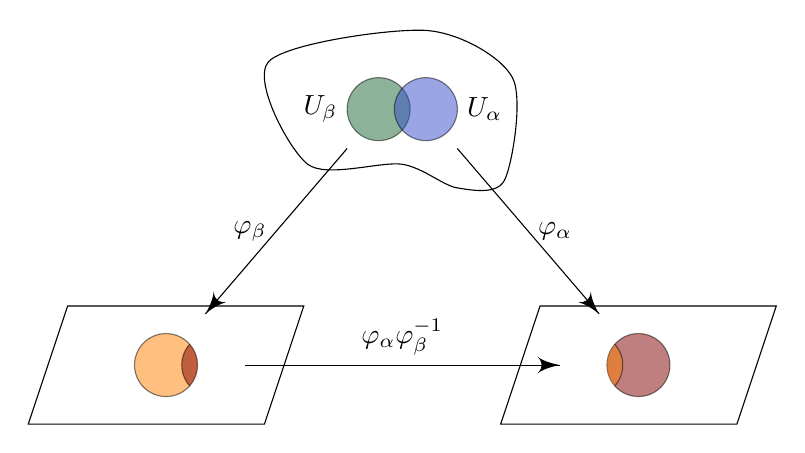
\begin{tikzpicture}
    \draw plot [smooth cycle] coordinates {(-1.2, -0.7) (0, -0.7) (0.7, -1) (1.3, -0.9) (1.4, 0.4) (0.3, 1) (-1.7, 0.6)};

    \draw (-0.3, 0) [fill=mgreen, opacity=0.5] circle [radius=0.4];
    \draw (0.3, 0) [fill=mblue, opacity=0.5] circle [radius=0.4];

    \node [left] at (-0.7, 0) {$U_\beta$};
    \node [right] at (0.7, 0) {$U_\alpha$};

    \begin{scope}[shift={(-4.75, -4)}]
      \draw (0, 0) -- (3, 0) -- (3.5, 1.5) -- (0.5, 1.5) -- cycle;

      \draw (1.75, 0.75) [fill=morange, opacity=0.5] circle [radius=0.4];
      \begin{scope}
        \clip (1.75, 0.75) circle [radius=0.4];
        \draw (2.35, 0.75) [fill=mred, opacity=0.5] circle [radius=0.4];
      \end{scope}
    \end{scope}

    \draw [->] (-0.7, -0.5) -- (-2.5, -2.6) node [pos=0.5, left] {$\varphi_\beta$};
    \draw [->] (0.7, -0.5) -- (2.5, -2.6) node [pos=0.5, right] {$\varphi_\alpha$};

    \begin{scope}[shift={(1.25, -4)}]
      \draw (0, 0) -- (3, 0) -- (3.5, 1.5) -- (0.5, 1.5) -- cycle;

      \draw (1.75, 0.75) [fill=mred, opacity=0.5] circle [radius=0.4];
      \begin{scope}
        \clip (1.75, 0.75) circle [radius=0.4];
        \draw (1.15, 0.75) [fill=morange, opacity=0.5] circle [radius=0.4];
      \end{scope}
    \end{scope}
    \draw [->] (-2, -3.25) -- (2, -3.25) node [pos=0.5, above] {$\varphi_\alpha \varphi_\beta^{-1}$};
  \end{tikzpicture}
\end{center}

As we consider differentiable (smooth) maps between two smooth manifolds $M$ and $N$, we can consider holomorphic maps between two complex manifolds $M$ and $N$. Let $M$ and $N$  be smooth manifolds, and let $\{(U_\alpha, \varphi_\alpha)\}_\alpha$ and $\{(V_\beta, \psi_\beta)\}_\beta$ be their  atlas. 

\begin{defi}[holomorphic map]\index{holomorphic map}
  A map $f: M \to N$ is \textbf{holomorphic} if, for a chart $(U_\alpha, \varphi_\alpha)$ of $p\in M$ and $(V_\beta, \psi_\beta)$ of $f(p)\in N$,  $ \psi_\beta \circ f \circ ( \varphi_\alpha)^{-1}: \varphi(U_\alpha \cap f^{-1} (V_\beta)) \to \xi(V_\beta )$ is holomorphic.


If there is the inverse map that is holomorphic, it is called a \term{biholomorphic} map, or $M$ and $N$ are \term{biholomorphic equivalent}.

\end{defi}
\begin{center}
  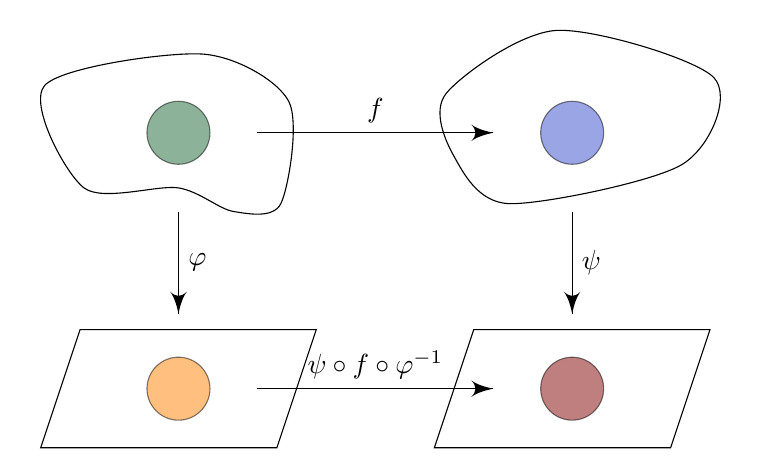
\begin{tikzpicture}
    \draw plot [smooth cycle] coordinates {(-1.2, -0.7) (0, -0.7) (0.7, -1) (1.3, -0.9) (1.4, 0.4) (0.3, 1) (-1.7, 0.6)};

    \draw [fill=mgreen, opacity=0.5] circle [radius=0.4];

    \begin{scope}[shift={(-1.75, -4)}]
      \draw (0, 0) -- (3, 0) -- (3.5, 1.5) -- (0.5, 1.5) -- cycle;

      \draw (1.75, 0.75) [fill=morange, opacity=0.5] circle [radius=0.4];
    \end{scope}

    \draw [->] (0, -1) -- +(0, -1.3) node [pos=0.5, right] {$\varphi$};
    \begin{scope}[shift={(5, 0)}]
      \draw plot [smooth cycle] coordinates {(1.4, -0.4) (-0.8, -0.9) (-1.5, -0.3) (-1.6, 0.5) (-0.2, 1.3) (1.8, 0.7)};

      \draw [fill=mblue, opacity=0.5] circle [radius=0.4];

      \begin{scope}[shift={(-1.75, -4)}]
        \draw (0, 0) -- (3, 0) -- (3.5, 1.5) -- (0.5, 1.5) -- cycle;

        \draw (1.75, 0.75) [fill=mred, opacity=0.5] circle [radius=0.4];
      \end{scope}

      \draw [->] (0, -1) -- +(0, -1.3) node [pos=0.5, right] {$\psi$};
    \end{scope}

    \draw [->] (1, 0) -- (4, 0) node [above, pos=0.5] {$f$};

    \draw [->] (1, -3.25) -- (4, -3.25) node [above, pos=0.5] {$\psi \circ f \circ \varphi^{-1}$};
  \end{tikzpicture}
\end{center}




\begin{eg}
Complex projective space $\CP^n$ is a complex manifold. (Check it satisfies the definition.)
\end{eg}



\begin{eg}
Let us now consider compact complex manifolds. It turns out that submanifolds of $\C^n$ are not  interesting, since a connected compact analytic submanifold of $\C^n$ is a point. However, many compact complex manifolds can be constructed as submanifolds of projective spaces $\CP^n$. We saw that $\CP^n$ is compact; all its closed complex submanifolds are also compact. In fact, there is a theorem by Chow stating that any compact submanifold of $\CP^n$ can be realized as the zero loci $F_i(z)=0$ of a finite number of homogeneous polynomial equations in the homogeneous coordinates $z_{\mu}$. These compact complex manifolds are called  \term{complex projective variety}. One important example is the \term{Fermat quintic} in $\CP^4$, given as the zero locus of the equation
\be
5\psi z_0z_1z_2z_3z_4-\sum_{\mu=0}^4 (z_{\mu})^5 = 0.
\ee
This three-dimensional compact complex manifold turns out to be \CY, probably the most studied \CY\ threefold because of mirror symmetry \cite{Candelas}. 
\end{eg}



\section{Holomorphic vector bundles}


\begin{defi}[Holomorphic vector bundle]\index{vector bundle}
  Let $M$ be a complex manifold and let $\pi: E \to M$ be a vector bundle of real rank $2r$
  \begin{enumerate}
    \item For each $p \in M$, the fiber $\pi^{-1}(p) = E_p$ is an $r$-dimensional complex vector space,
    \item For all $p \in M$, there is an open $U \subseteq M$ containing $p$ and a diffeomorphism
      \[
        t: E_U = \pi^{-1}(U) \to U \times \C^r
      \]
      such that
      \[
        \begin{tikzcd}
          E_U \ar[r, "t"] \ar[d, "\pi"] & U \times \C^r \ar[dl, "p_1"]\\
          U
        \end{tikzcd}
      \]
      commutes, and the induced map $E_q \to \{q\} \times \C^r$ is a linear isomorphism for all $q \in U$.
     \item 
  Suppose that $t_\alpha: E|_{U_\alpha} \to U_\alpha \times \C^r$ and $t_\beta: E|_{U_\beta} \to U_\beta \times \C^r$ are trivializations of $E$. Then
  \[
    t_\alpha \circ t_\beta^{-1} : (U_\alpha \cap U_\beta) \times \C^r \to (U_\alpha \cap U_\beta) \times \C^r
  \]
  is fiberwise linear, i.e.
  \[
    t_\alpha \circ t_\beta^{-1}(q, v) = (q, g_{\alpha\beta}(z) v),
  \]
  where $g_{\alpha\beta}(z):U_\alpha \cap U_\beta\to \GL(r,\C)$ is a holomorphic function.
The transition functions have the following properties
  \begin{enumerate}
    \item $g_{\alpha\alpha} = \id$
    \item $g_{\alpha\beta} = g_{\beta\alpha}^{-1}$
    \item $g_{\alpha\beta}g_{\beta\gamma} g_{\gamma\alpha}= 1$.
  \end{enumerate}
  \end{enumerate}
\end{defi}


\subsection{Holomorphic tangent and cotangent bundle}
Let $(U,(z_1,\cdots,z_n))$ be a local coordinate of a complex manifold $M$ and we decompose the complex coordinate $z_j=x_j+iy_j$ into the real and imaginary part. Then, the basis of the tangent bundle $TM$ on an open set $U\subset M$ can be taken by $\frac\partial{\partial x_j}$, $\frac\partial{\partial y_j}$ ($j=1,\cdots,n$). Now let us complexify the tangent bundle $T_{\C} M:=TM\otimes \bC$ where we can take the basis on $U$ as
$$
\frac\partial{\partial z_j}:=\frac12\Big(\frac\partial{\partial x_j}-i\frac\partial{\partial y_j}\Big)~,\qquad \frac\partial{\partial \overline z_j}:=\frac12\Big(\frac\partial{\partial x_j}+i\frac\partial{\partial y_j}\Big)~.
$$
Each fiber of $T_pM\otimes \C$ is a vector space with basis  $\frac\partial{\partial x_j}$, $\frac\partial{\partial y_j}$ on $\C$. Similarly, one can complexify the cotangent bundle $T_{\C}^* M:=T^*M\otimes \C$ where we can take basis $dz_j$, $d\overline z_j$ on $U$. At each point $p\in M$, we can take the subspace $T^{(1,0)}_p M$ of $T_p M\otimes \C$ spanned by $\{\frac\partial{\partial z_j}\}$. A family of the subspace is denoted by $T^{(1,0)} M =\cup_p T^{(1,0)}_p M$ and we can also define $T^{*(1,0)} M =\cup_p T^{*(1,0)}_p M$ in a similar fashion. Given another chart $(V(w_1,\cdots,w_n))$, they transform 
$$
\frac\partial{\partial z_j}=\frac{\partial w_k}{\partial z_j}\frac\partial{\partial w_k}~, \quad dz_j=\frac{\partial z_j}{\partial w_k}dw_k
$$ 
where the transition functions $\frac{\partial w_k}{\partial z_j}$ and $\frac{\partial z_j}{\partial w_k}$ are holomorphic so that they are holomorphic vector bundles. Indeed, we can decompose complxified (co)tangent bundle as
$$T_{\C} M = T^{(1,0)} M \oplus T^{(0,1)} M~,\qquad T_{\C}^* M = T^{*(1,0)} M \oplus T^{*(0,1)} M~.$$
We call $T^{(1,0)} M$ (resp. $T^{(0,1)} M$) the \term{holomorphic (resp. anti-holomorphic) (co)tangent bundle}. 


As a real bundle. $T^{(1,0)} M$ is isomorphic to $T M$. In fact, We can define a map $\textrm{Re}:T_\C M\to TM$ by taking real part
$$
2\textrm{Re}~\frac\partial{\partial z_j}=\frac\partial{\partial x_j}~,
$$ 
 which is an isomorphism. Since $T^{(1,0)} M$ is a complex vector bundle, we have the multiplication by $i$, which induces an isomorphism $J:TM\to TM$:
 $$
 2\textrm{Re}~\frac\partial{\partial z_j}=\frac\partial{\partial x_j}~,\quad  2\textrm{Re}~ i\frac\partial{\partial z_j}=\frac\partial{\partial y_j}~,
 $$
 so that
 $$
 J\Big( \frac\partial{\partial x_j}\Big)= \frac\partial{\partial y_j}~,\quad  J\Big( \frac\partial{\partial y_j}\Big)= -\frac\partial{\partial x_j}~.
 $$
It is easy to check $J^2=-\textrm{id}_{TM}$, and  the eigenvalues of $J$ in $T_pM \otimes \C$ are $\pm i$. Hence, we consider $T^{(1,0)}_p M$ (resp. $T^{(0,1)}_p M$) as the eigenspace of $J_p$ with eigenvalue $i$ (resp. $-i$). $J$ is called \term{almost complex structure}.
 
 An almost complex structure $J_M:TM\to TM$ is a complex structure if for any $p\in m$ there exist an open neighborhood $p\in U\subset M$, $V\subset \C^n$, and a continuous map $\varphi:U\to V$ such that $d\varphi\cdot J_M=J_{\C^n}\cdot d\varphi$. If an almost complex structure $J_M$ is a complex structure, $J_M$ is called to be \term{integrable}. The Newlander-Nirenberg theorem states that an almost complex structure $J$ is integrable if and only if the Nijenhuis tensor vanishes:
 $$
 N_{J}(X,Y)=-J^{2}[X,Y]+J([JX,Y]+[X,JY])-[JX,JY]=0~$$
 for ${}^\forall X,Y\in \mathfrak{X}(M)$.
 
 
 The only spheres which admit almost complex structures are $S^2$ and $S^6$. In particular, $S^4$ cannot be given an almost complex structure. In the case of $S^2$, the almost complex structure comes from the complex structure of the Riemann sphere. The 6-sphere $S^6$ inherits an almost complex structure from the octonion multiplication;. However, whether $S^6$ has a complex structure is an open question.

\subsection{Differential forms}
Locally, any differential forms can be expressed as a linear combination of the exterior products of $dz_j$ and $d\overline z_k$. In particular, a differential form which can be expanded in terms of
$$
dz_{i_1}\wedge \cdots \wedge dz_{i_p}\wedge d\overline z_{i_1}\wedge \cdots \wedge d\overline z_{i_q}
$$
called $(p,q)$-form, which is a section of $\bigwedge^p T^{*(1,0)} M \otimes \bigwedge^{q} T^{*(0,1)} M$. We denote the vector space of $(p,q)$-forms by $\Omega^{p,q}(M)$.
In fact,  it is easy to show that the following complexified bundles decompose as
$$
\bigwedge^k T^*_{\C} M = \bigoplus_{j=0}^k \bigwedge^j T^{*(1,0)} M \otimes \bigwedge^{k-j} T^{*(0,1)} M,
$$

On a complex manifold, the exterior derivative also admits a simple decomposition: $d = \partial + \bar{\partial}$, where we defined the operators 
$$\partial: \Omega^{p,q}(M) \to \Omega^{p+1,q}(M)~,\qquad \bar{\partial}: \Omega^{p,q}(M) \to \Omega^{p,q+1}(M)~.$$
The identity $d^2=0$ implies that $\partial^2=\bar{\partial}^2=0$ and $\partial \bar{\partial}+\bar{\partial} \partial=0$. 
%We can also define a real operator $d^c: \Omega^k_{\C} (M) \to \Omega^{k+1}_{\C} (M)$ by $d^c = i (\bar{\partial}-\partial)$, which satisfies
%\be
%d d^c + d^c d=0,~~~(d^c)^2=0,~~~\partial = \frac12 (d+id^c),~~~\bar{\partial} = \frac12 (d-id^c),~~~d d^c = 2i \partial \bar{\partial}.
%\ee

A $(p,0)$-form is an element of $\Omega^{p,0}(M)$ and it can be locally written as
$$
\varphi=\sum \varphi_{i_1, \cdots  ,i_p}(z)dz_{i_1}\wedge \cdots \wedge dz_{i_p}
$$
where $\varphi_{i_1, \cdots  ,i_p}(z)$ is holomorphic. Therefore, $\phi$ is called \term{a holomorphic $p$-form}. In particular, when $p=n$, 
$$
K_M=\bigwedge^n  T^{*(1,0)} M
$$
is called \term{the canonical line bundle}. Since $TM$ is isomorphic to $ T^{(1,0)} M$, the first Chern class is
$$
c_1(M)=c_1(TM)=c_1(T^{(1,0)} M)=c_1(\bigwedge^n  T^{(1,0)} M)=-c_1(K_M)
$$


Now what is the analog of the de Rham cohomology groups for complex manifolds? 

\begin{defi}
Let $M$ be a complex manifold of complex dimension $m$. As $\bar{\partial}^2=0$, we can form the complex
$$
\begin{array}{ccccccccccc}
&\bar{\partial}&&\bar{\partial}&&\bar{\partial}&&\bar{\partial}&&\bar{\partial}&\\
0 &\to& \Omega^{p,0}(M) &\to& \Omega^{p,1}(M) &\to& \ldots &\to& \Omega^{p,n}(M) &\to&0.
\end{array}
$$
We define the \term{Dolbeault cohomology groups} $H^{p,q}_{\bar{\partial}} (M)$ of $M$ by
$$
H^{p,q}_{\bar{\partial}} (M) = {{\rm Ker}(\bar{\partial}: \Omega^{p,q}(M) \to \Omega^{p,q+1}(M)) \over {\rm Im} (\bar{\partial}: \Omega^{p,q-1}(M) \to \Omega^{p,q}(M))}.
$$
\end{defi}

Remark that the Dolbeault cohomology groups depend on the complex structure of $M$. Note also that we could have defined the cohomology groups using $\partial$ instead of $\bar{\partial}$, this is just a matter of convention since they are complex conjugate. 

\begin{thm}[Hodge decomposition theorem for K\"ahler manifolds]
For a compact K\"ahler manifold $M$, the complex cohomology satisfies
\begin{align}
H^r(M, \C) \cong \bigoplus_{p+q=r}H^{p,q}_{\bar{\partial}} (M) ~,\cr
H^{p,q}_{\bar{\partial}} (M) =\overline{H^{q,p}_{\bar{\partial}} (M)}
\end{align}
where $H^{p,q}_{\bar{\partial}} $
is the Dolbeault cohomology restricted to forms of type $(p, q)$. Further, we could
instead choose the de Rham cohomology to obtain the same result, and the cohomology classes
contain unique harmonic representatives. Consequently, holomorphic forms are therefore
harmonic for any K\"ahler  metric on a compact manifold, and the odd Betti numbers are
even.
\end{thm}


We now define the \term{Hodge numbers}  to be $h^{p,q} = \dim H^{p,q}_{\bar{\partial}} (M)$. The Hodge numbers of a complex manifold are summarized in what is commonly called the \term{Hodge diamond}:
$$
\begin{array}{ccccc}
&&h^{n,n}&& \\
&h^{n,n-1}&\vdots&h^{n-1,n}& \\
h^{n,0}&\cdots&&\cdots&h^{0,n}\\
&h^{1,0}&\vdots&h^{1,0}& \\
&&h^{0,0}&& \\
\end{array}
$$



\begin{thm}[Hard Lefschetz Theorem] Let $(M, \omega)$ be a K�ahler manifold. Let $L$ be
exterior multiplication by the K\"ahler form $\omega$. Then
$$L^k: H^{n-k}(M) \to H^{n+k}(M)$$
is an isomorphism for $1 \le k \le n$. Further, if we define the primitive cohomology $P^j(M)$ by
$$P^j(M) = \ker L^{n-j+1} : H^j \to H^{2n-j+2}~,$$
then we have the Lefschetz decomposition
$$H^m (M) = \bigoplus_k L^k P^{m-2k}(M)~.$$
Thus, the Betti numbers of a compact K\"ahler manifold have a pyramid structure, called the
\term{Hodge pyramid}.
\end{thm}











\section{K\"ahler manifolds}

The condition for a Riemannian metric $g$ to be Hermitian is that for ${}^\forall X,Y\in \mathfrak{X}(M)$, and ${}^\forall \alpha,\beta\in\C$,  it satisfies
$$
g(\alpha X,\beta y)= \alpha \overline\beta g(X,Y)~.
$$
This condition amounts to the case when $\alpha=\beta=i$. Since the multiplication by $i$ corresponds to $J$, the Hermitian metric can be defined as follows.

\begin{defi}
Let $(M,J)$ be a complex manifold, and let $g$ be a Riemannian metric on $M$. We call $g$ a \term{Hermitian metric} if $g(v,w) = g(Jv,Jw)$ for all vector fields $v,w$ on $M$
%\item{In component notation, $g_{ab} = J_a^c J_b^d g_{cd}$;}
%\item{Using the greek indices notation, $g_{ab}=g_{\alpha \bar{\beta}}+g_{\bar{\alpha} \beta}$, that is $g_{\alpha \beta} = g_{\bar{\alpha} \bar{\beta}} = 0$.}
%\end{enumerate}
\end{defi}


In other words, a Hermitian metric is a positive-definite inner product $T^{(1,0)}M \otimes T^{(0,1)} M \to \C$ at every point on a complex manifold $M$. In local coordinate, we can express $g$ on $T_\C M$ by
$$
g_{j\overline k}=g\Big(\frac\partial{\partial z_j},\frac\partial{\partial \overline z_k} \Big)~,
$$
so that $g_{j\overline k}$ is a Hermitian metric.

Using this Hermitian metric $g$, we can define a two-form $\omega$ on $M$ called the \term{Hermitian form} by $\omega(v,w) = g(Jv, w)$ for all vector fields on $v,w$ on $M$. In local coordinate, it can be written as
$$
\omega=i g_{j\overline k}dz_j\wedge d\overline z_k
$$
Therefore, $\omega$ is a $(1,1)$-form. 



\begin{defi}
Let $(M,J)$ be a complex manifold, and $g$ a Hermitian metric on $M$, with Hermitian form $\omega$. $g$ is a \term{K\"ahler metric} if $d \omega= 0 $. In this case we call $\omega$ a \term{K\"ahler form}, and we call a complex manifold $(M,J)$ endowed with a K\"ahler metric a \term{K\"ahler manifold}.
\end{defi}



\begin{thm}
Any complex submanifold $N\subset M$ of a K\"ahler manifold $(M,\omega)$ is K\"ahler where the K\"ahler form is its restriction $\omega_N=\omega\Big|_N$.
\end{thm}

For a K\"ahler manifold $M$, the holonomy group is $U(n) \subset SO(2n)$.
The condition that a Riemannian metric $g$ can be K\"ahler is equivalent to $\nabla J=0$ with respect to Levi-Civita connection of $g$.
In addition, it can be shown that locally, the K\"ahler condition $d \omega= 0$ is equivalent to the condition $\partial_{\ell} g_{j\overline k} = \partial_{j} g_{\ell\overline k}$ and its conjugate equation $\overline\partial_{\bar{\ell}} g_{j\overline k} =\overline \partial_{\bar{k}} g_{j \bar{\ell}}$. Locally, we can always integrate these equations as,
$$g_{j\overline k}=  \partial_j \bar{\partial}_{\overline k} K ( z , \overline z ) ,$$
for some function $ K ( z , \overline z )$, which is known as the  \term{K\"ahler potential}. It is unique up to  K\"ahler 
transformation, $ K ( z , \overline z )\to K ( z , \overline z )+f(z)+f(\overline z)$ for any holomorphic function $f(z)$. We should
note that the  K\"ahler  potential cannot be a globally defined smooth function on a compact   manifold $M$.


 Since $\omega$ is closed, it defines a Dolbeault cohomology class $[\omega] \in H^{1,1}_{\bar{\partial}} (M)$, or a de Rham cohomology class $[\omega] \in H^2_{dR} (M, \R)$.  Further, the wedge product of $n$ copies of $\omega$, denoted by $\omega^n$, is proportional to the volume form of $g$. Therefore it defines a non-trivial element in both $H^{n,n}_{\bar{\partial}} (M)$ and $H^{2n}_{dR} (M,\R)$ so that $[\omega]$ must be non-trivial. However, $ \partial_j \bar{\partial}_{\overline k} K ( z , \overline z ) $ is exact and therefore zero as a cohomology class. It follows that on a compact K\"ahler manifold it is impossible to define a K\"ahler potential globally.
 
 
 
 
\begin{eg}
Complex projective space $\CP^n$ is a K\"ahler manifold.  Consider the function $u(z_0,\cdots,z_m) = \sum_{\mu=0}^n |z_\mu|^2$ where $z_\mu$, $\mu=0,\cdots,n$ are homogeneous coordinates on $\C^{n+1} \backslash \{0\}$. Define a $(1,1)$-form $\alpha$ by $\alpha =\partial \overline\partial (\log u)$. $\alpha$ cannot be the K\"ahler form of any metric on $\C^{n+1} \backslash \{0\}$, since it is not positive. However, if we consider the projection $\pi: \C^{n+1} \backslash \{0\} \to \CP^n$ defined by $\pi: (z_0,\cdots,z_n) \mapsto [z_0;\cdots;z_n]$, one can show that there exists a unique positive $(1,1)$-form $\omega$ on $\CP^n$ such that $\alpha = \pi^* (\omega)$. $\omega$ is a K\"ahler form on $\CP^n$; its associated K\"ahler metric is called the \term{Fubini-Study metric}, and is given in components by $g_{\mu \bar{\nu}} = \partial_j \overline\partial_{\bar{k}} \log u$.
$$
\omega_{\textrm{FS}}=i\frac{\sum_j dz_j\wedge d\overline z_j-\sum_{k ,j}(\overline  z_j d z_j)\wedge (z_k d\overline z_k) }{(|z_0|^2+\cdots+|z_n|^2)^2}~.
$$
\end{eg}



Given the metric in the above form, we can compute the Riemann curvature.
Straightforward calculations show that the only non-zero components are $\Gamma^i_{j k} = g^{i \overline \ell} \partial_j g_{ k \overline \ell} $,
and its complex conjugate. Thus, the only non-zero components of the curvature tensor are
$R^\ell {}_{ i \overline j k} = \partial_{\overline j} \Gamma^\ell_{ik}$.
Furthermore, the Ricci tensor turns out to be
$$
R_{j\overline k}=R^\ell {}_{ \ell  j \overline k} =i\partial_j \overline\partial_{\overline k} \log\det (g)~.
$$


For a K\"ahler manifold, the complexified de Rham cohomology decomposes into the Dolbeault cohomology (note that the de Rham cohomology groups are complex, as we are now considering complexified $k$-forms)
$$
H^k_{dR} (M, \C) = \bigoplus_{j=0}^k H^{j,k-j}_{\bar{\partial}} (M).
$$
This can be shown by using Hodge theorem of  a K\"ahler manifold.

\section{\CY \  manifolds}

We are now ready to study \CY\ manifolds, which are a particular kind of K\"ahler manifolds.

In 1954,  Calabi conjectured that a compact K\"ahler manifold $M$ with $c_1=0$ admits Ricci-flat K\"ahler metric.  Yau proved the conjecture in 1976 by solving the complex Monge-Amp�re equation.  Therefore, such a manifold is called a \term{\CY\ manifold}.
%
%However, many different definitions of \CY\ manifolds exist in the literature; we will review some of the most common definitions and study some relations among them. We will also investigate properties of \CY\ manifolds and study in details a few examples. We will end this section by quickly describing `local' \CY\ manifolds (i.e. noncompact \CY\ manifolds), which have many applications for instance in topological strings and Gromov--Witten theory.

\CY\ manifolds have been studied extensively in the recent decades, particularly because of their importance in string theory \cite{Calabi-Yau}. While the mathematical study of \CY\ manifolds has helped us understand compactifications of string theory, the study of string theory has led to fascinating insights in the geometry of \CY\ manifolds, for example the study of the \CY\ moduli space and mirror symmetry. \CY\ manifolds are thus a very good example of the fruitful interactions between mathematics and physics that have been taking place in the recent decades.

%\subsection{\CY\ manifolds}

Let us first list some of the most common definitions of \CY\ manifolds. A \CY\ manifold of real dimension $2n$ is a compact K\"ahler manifold $(M,J,g)$: 
\begin{enumerate}
\item{with zero Ricci form,}
\item{with vanishing first Chern class,}
\item{with ${\rm Hol}(g) = SU(n)$ (or ${\rm Hol}(g) \subseteq SU(n)$),}
\item{with trivial canonical bundle,}
\item{that admits a globally defined and nowhere vanishing holomorphic $n$-form.}
\end{enumerate}

 


The Hodge numbers of a \CY\ manifold satisfy a few more properties, which drastically decrease the number of undetermined Hodge numbers. We will now focus on \CY\ threefolds, that is \CY\ manifolds with complex dimension $3$, for the sake of brevity. These are the most important \CY\ manifolds in string theory applications. But most results extend straighforwardly to higher dimensional \CY\ manifolds.

The Hodge numbers of K\"ahler manifolds satisfy a Hodge star duality $h^{p,q} = h^{3-q,3-p}$ and a complex conjugation duality $h^{p,q}=h^{q,p}$. For \CY\ manifolds, there is a further duality, sometimes called \term{holomorphic duality}. The triviality of the canonical bundle of a \CY\ manifold $M$ implies that $h^{3,0} = 1$, i.e. the existence of a unique holomorphic volume form $\Omega$. Given a $(0,q)$ cohomology class $[\alpha]$, there is a unique $(0,3-q)$ cohomology class $[\beta]$ such that $\int_M \alpha \wedge \beta \wedge \Omega = 1$ (using Stoke's theorem). Thus $h^{0,q} = h^{0,3-q}$. Therefore, for a \CY\ manifold we have that $h^{3,0}=h^{0,3}=h^{0,0}=h^{3,3}=1$.

Moreover, one can show that $h^{1,0}=0$. Thus, $h^{1,0}=h^{0,1}=h^{0,2}=h^{2,0}=h^{2,3}=h^{3,2}=h^{3,1}=h^{1,3}=0$. Therefore, the only remaining independent Hodge numbers are $h^{1,1}$ and $h^{2,1}$, and the Hodge diamond takes the form:
$$
\begin{array}{ccccccc}
&&&1&&& \\
&&0&&0&& \\
&0&&h^{1,1}&&0&\\
1&&h^{2,1}&&h^{2,1}&&1\\
&0&&h^{1,1}&&0&\\
&&0&&0&& \\
&&&1&&& \\
\end{array}
$$

The Euler characteristic of a \CY\ manifold accordingly simplifies. Recall that $\chi = \sum_{k=0}^{2m} (-1)^k b^k$, so we now have that $\chi=2b^0-2b^1+2b^2-b^3 = 2-0+2h^{1,1}-2-2h^{2,1}$, that is
$$
\chi = 2(h^{1,1}-h^{2,1}).
$$

Therefore, if the Euler characteristic is easily computed, we only have to compute one of the two independent Hodge numbers to get all the topological information. In fact,  the Euler characteristic is given by the integral over $M$ of the top Chern class of $M$, which is $c_3(M)$ for a \CY\ threefold:
$$
\chi = \int_M c_3(M).
$$
This formula can be used to compute the Euler characteristic of $M$. 

The Hodge number $h^{1,1}$ classifies infinitesimal deformations of the K\"ahler structure that, roughly speaking, parametrizes the volume of $M$. For a \CY\ threefold, $h^{2,1}$ classifies infinitesimal deformations of the complex structure that, roughly speaking, parametrizes the shape of $M$. 


One of the fascinating property of \CY\ threefolds is that they come in mirror pairs, $(M,W)$, such that $H^{2,1} (W) \cong H^{1,1} (M)$ and $H^{1,1} (W) \cong H^{2,1} (M)$. Roughly speaking, the complex structure moduli is exchanged with the K\"ahler structure moduli. This is the basic idea behind \term{mirror symmetry}. 

\subsection{Examples}
\begin{eg}
A torus $T^2$ is a compact \CY\ manifold one-fold. The Hodge diamond of $T^2$ is
$$
\begin{array}{cccc}
&1&\\
1&&1\\
&1&
\end{array}
$$
The moduli space of the complex structure is written below.
\end{eg}

\begin{figure}[h]\centering
\includegraphics[width=10cm]{modular}
\end{figure}

\begin{eg}
$T^4$ is a compact \CY\ manifold 2-fold. The Hodge diamond of $T^4$ is
$$
\begin{array}{cccccc}
&&1&&\\
&2&&2&\\
1&&4&&1\\
&2&&2&\\
&&1&&
\end{array}
$$
\end{eg}


\begin{eg}
The other compact \CY\ 2-fold is a K3 surface, which is constructed as follows. Let us consider the quotient space $T^4/\Z_2$. There are 16 singular points and the neighborhood around a singular point is a cone of $\RP^3$. If we consider the set $V=\{p\in TS^2| ~|v|\le1\}$ of points with length $\le1$ in a fiber of $TS^2$, its boundary is $\partial V\cong\RP^3$. Therefore, we can replace the neighborhood of each singular point by $V$. Then, the resulting space is smooth and it is a K3 surface. The Hodge diamond of a K3 surface is
$$
\begin{array}{cccccc}
&&1&&\\
&0&&0&\\
1&&20&&1\\
&0&&0&\\
&&1&&
\end{array}
$$
\end{eg}






\begin{eg}
As mentioned before, a submanifold $\CP^4$ defined by
$$
M=\{z_0^5+z_1^5+z_2^5+z_3^5+z_4^5-5\psi z_0z_1z_2z_3z_4=0\}
$$
is a compact \CY\ 3-fold. Let us define the group
$$
G = \{(a_0,\cdots , a_4) \in (\Z_5)^5|\sum_ia_i = 0\}/(\Z_5 = \{(a, a, a, a, a)\}).
$$
Then, the mirror manifold $W$ is constructed by the resolution of singularities of  the orbifold $M/G$ where $G$ acts on $M$ by $ (z_j ) \to (z_j \omega^{a_j} )$ with $\omega=e^{2\pi i/5}$.
The Hodge diamonds of $M$ and $W$ are given by

\begin{minipage}[b]{6.5cm}
$$\begin{array}{ccccccc}
&&&1&&&\\	
&&0	&&0&&\\	
&0&&1&&	0&\\
1&&101&&101&&1\\
&0&&1&&0&\\
&&0	&&0	&&\\
&&&1&&&		
\end{array}$$
\quad \qquad {Hodge diamonds of $M$}
\end{minipage}
\begin{minipage}[b]{6.5cm}
$$\begin{array}{ccccccc}
&&&1&&&\\	
&&0	&&0&&\\	
&0&&101&&	0&\\
1&&1&&1&&1\\
&0&&101&&0&\\
&&0	&&0	&&\\
&&&1&&&		
\end{array}$$
\qquad \quad {Hodge diamonds of $W$}
\end{minipage}
\\

\noindent where you can see the mirror symmetry.
\end{eg}



\begin{thebibliography}{99}

\bibitem{Candelas}
P. Candelas, X. C. de La Ossa, P. S. Green, L. Parkes, \textit{A pair of Calabi-Yau manifolds as an exactly soluble superconformal theory}. Nucl.Phys. B359 (1991) 21-74.

\bibitem{Bouchard}
Vincent. Bouchard,  \textit{Lectures on complex geometry, Calabi-Yau manifolds and toric geometry.} \href{http://arxiv.org/abs/hep-th/0702063}{hep-th/0702063} (2007).

\bibitem{Calabi-Yau}
Calabi-Yau manifolds, 
\url{http://www.scholarpedia.org/article/Calabi-Yau_manifold}

\end{thebibliography}


\end{document}
